    
    

    
\section{Performance of Layer 5 Prefrontal cortex Pyramidal Neuron on
NeuronUnit tests of model data
agreement}
    \begin{verbatim}[commandchars=\\\{\}]
 \{'value': array(196.875) * pA\}
    \end{verbatim}

    \begin{center}
    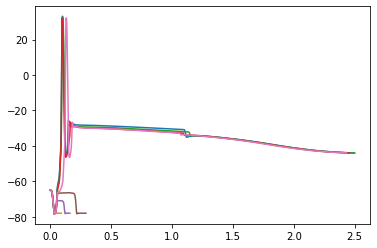
\includegraphics[width=0.7\linewidth]{figures/NU_BBP_fusion_L5PC_files/NU_BBP_fusion_L5PC_3_1.png}
    \end{center}

    \begin{verbatim}
5.74 s +- 34.8 ms per loop (mean +- std. dev. of 7 runs, 1 loop each)
    \end{verbatim}

    \begin{center}
    \adjustimage{max size={0.9\linewidth}{0.9\paperheight}}{NU_BBP_fusion_L5PC_files/NU_BBP_fusion_L5PC_4_1.png}
    \end{center}
    { \hspace*{\fill} \\}
    
    \begin{Verbatim}[commandchars=\\\{\}]
22.9 s ± 1.33 s per loop (mean ± std. dev. of 7 runs, 1 loop each)
    \end{Verbatim}

    \begin{center}
    \adjustimage{max size={0.9\linewidth}{0.9\paperheight}}{NU_BBP_fusion_L5PC_files/NU_BBP_fusion_L5PC_4_3.png}
    \end{center}
    { \hspace*{\fill} \\}
    
    \begin{Verbatim}[commandchars=\\\{\}]
The slowest run took 5.32 times longer than the fastest. This could mean that an
intermediate result is being cached.
40.6 s ± 27.5 s per loop (mean ± std. dev. of 7 runs, 1 loop each)
    \end{Verbatim}

    \begin{center}
    \adjustimage{max size={0.9\linewidth}{0.9\paperheight}}{NU_BBP_fusion_L5PC_files/NU_BBP_fusion_L5PC_4_5.png}
    \end{center}
    { \hspace*{\fill} \\}
    
    \begin{Verbatim}[commandchars=\\\{\}]
12.9 s ± 3.04 s per loop (mean ± std. dev. of 7 runs, 1 loop each)
    \end{Verbatim}

    \begin{center}
    \adjustimage{max size={0.9\linewidth}{0.9\paperheight}}{NU_BBP_fusion_L5PC_files/NU_BBP_fusion_L5PC_5_1.png}
    \end{center}
    { \hspace*{\fill} \\}
    
    \begin{Verbatim}[commandchars=\\\{\}]
1000.0 ms 100.0 ms
    \end{Verbatim}

            \begin{tcolorbox}[breakable, size=fbox, boxrule=.5pt, pad at break*=1mm, opacityfill=0]
\begin{Verbatim}[commandchars=\\\{\}]
                                        observations             predictions  \textbackslash{}
RheobaseTest                     213.849583333333 pA                225.0 pA
RestingPotentialTest            -68.2481434599156 mV   -78.04177135432035 mV
InjectedCurrentAPWidthTest       1.20769387755102 ms   1.9430908350894676 ms
InjectedCurrentAPAmplitudeTest   80.4351020408164 mV    63.58198269900037 mV
InjectedCurrentAPThresholdTest  -42.7357232704403 mV  -33.316186032597116 mV

                                 Z-Scores
RheobaseTest                     Z = 0.07
RestingPotentialTest            Z = -1.50
InjectedCurrentAPWidthTest       Z = 1.38
InjectedCurrentAPAmplitudeTest  Z = -1.32
InjectedCurrentAPThresholdTest   Z = 1.17
\end{Verbatim}
\end{tcolorbox}
        
            \begin{tcolorbox}[breakable, size=fbox, boxrule=.5pt, pad at break*=1mm, opacityfill=0]
\begin{Verbatim}[commandchars=\\\{\}]
'\textbackslash{}nscores = [] \textbackslash{}nfor i,t in enumerate(nu\_tests):\textbackslash{}n    try:\textbackslash{}n        score =
t.judge(l5)\textbackslash{}n        scores.append(score)\textbackslash{}n    except:\textbackslash{}n        del
nu\_tests[i]\textbackslash{}n'
\end{Verbatim}
\end{tcolorbox}
        
    \hypertarget{neocortical-layer-45-pyramidal-cell-test-suite}{%
\section{Neocortical Layer 4/5 Pyramidal Cell Test
Suite}\label{neocortical-layer-45-pyramidal-cell-test-suite}}

\begin{table}[]
\begin{tabular}{|l|l|l|l|l|}
\hline
TestType & experimental-observation & model-prediction& Z-score &  \\ \hline
c & d &  &  &  \\ \hline
  &   &  &  &  \\ \hline
  &   &  &  &  \\ \hline
\end{tabular}
\end{table}    
    
    \begin{verbatim}
  RheobaseTest RestingPotentialTest InjectedCurrentAPWidthTest  \
0     Z = 0.07            Z = -1.50                   Z = 1.38   

  InjectedCurrentAPAmplitudeTest InjectedCurrentAPThresholdTest  
0                      Z = -1.32                       Z = 1.17  
    \end{verbatim}

    
    \begin{Verbatim}[commandchars=\\\{\}]

        ---------------------------------------------------------------------------

        TypeError                                 Traceback (most recent call last)

        <ipython-input-9-ca1ec313471d> in <module>
          3 SA\_nc = ScoreArray(l5pc\_tests, scores\_nc)
          4 display(SA\_nc.to\_frame().T)
    ----> 5 obs\_preds\_nc = make\_pretty(l5pc\_tests)
          6 display(obs\_preds\_nc.T)


        TypeError: make\_pretty() missing 1 required positional argument: 'scores\_nc'

    \end{Verbatim}

    \hypertarget{get-rid-of-all-besides-one-protocol-then-hijack-the-last-one-to-fit-our-purposes.}{%
\section{get rid of all besides one protocol, then hijack the last one
to fit our
purposes.}\label{get-rid-of-all-besides-one-protocol-then-hijack-the-last-one-to-fit-our-purposes.}}


